% !TeX TS-program = xelatex
\documentclass[12pt]{article}
\usepackage{listings}
\usepackage{float}
\usepackage{xcolor}
\usepackage{graphicx}
\definecolor{codegreen}{rgb}{0,0.6,0}
\definecolor{codegray}{rgb}{0.5,0.5,0.5}
\definecolor{codepurple}{rgb}{0.58,0,0.82}
\definecolor{backcolour}{rgb}{0.95,0.95,0.92}
\lstdefinestyle{mystyle}{
	backgroundcolor=\color{backcolour},   commentstyle=\color{codegreen},
	keywordstyle=\color{magenta},
	numberstyle=\tiny\color{codegray},
	stringstyle=\color{codepurple},
	basicstyle=\ttfamily\footnotesize,
	breakatwhitespace=false,
	breaklines=true,
	captionpos=b,
	keepspaces=true,
	numbers=left,
	numbersep=5pt,
	showspaces=false,
	showstringspaces=false,
	showtabs=false,
	tabsize=2
}
%"mystyle" code listing set
\lstset{style=mystyle}
%\lstset{basicstyle=\ttfamily\footnotesize,breaklines=true}

\usepackage[breaklinks]{hyperref}
% Setup de hiperenlaces
\hypersetup{
	colorlinks=true,
	linkcolor=blue,
	filecolor=magenta,
	urlcolor=cyan,
	pdftitle={Apuntes de Consolas y Videojuegos},
	pdfpagemode=FullScreen,
	citecolor = green
}

\usepackage{url}

\usepackage{fontspec}
\setmainfont{AT-NameSansText}[
	Path=./NameSansStatic/,
	Extension = .otf,
	UprightFont=*-Regular,
	BoldFont=*-Bold,
	ItalicFont=*-RegularItalic,
	BoldItalicFont=*-BoldItalic,
	Numbers = OldStyle
]

\setmonofont{ATNameMono}[
	Path=./NameMonoStatic/,
	Extension = .otf,
	UprightFont=*-Regular,
	BoldFont=*-Bold,
	ItalicFont=*-RegularItalic,
	BoldItalicFont=*-BoldItalic
]

\usepackage{biblatex}
\addbibresource{referencias.bib}
\usepackage{notoccite}


\begin{document}
\nocite{namesans_about}
\nocite{namesans}
\nocite{namemono}


	\begin{titlepage}
		\begin{center}
			{\Huge \textbf{Ejercicios Ensamblador Hack}} 

			\vspace{2cm}

			{\Large \textit{Jesús Jiménez Montero}}

			\vspace{2cm}

			\textbf{Versión 1}: Entregable 7
		\end{center}
	\end{titlepage}

	% ÍNDICE
	%\renewcommand{\tableofcontents}{Indice general}
	\newpage
	\renewcommand{\contentsname}{Tabla de contenidos}
	\setcounter{secnumdepth}{5}
	\tableofcontents
	\setcounter{tocdepth}{4}
	\newpage

	\section{Entregable 7}
		\subsection{Ejercicio 1}
			\begin{lstlisting}

				// Suma numeros 3+4+7
				@3
				D = A
				@4
				D = D + A
				@7
				D = D + A
			\end{lstlisting}

			% TODO: \usepackage{graphicx} required
			\begin{figure}[H]
				\centering
				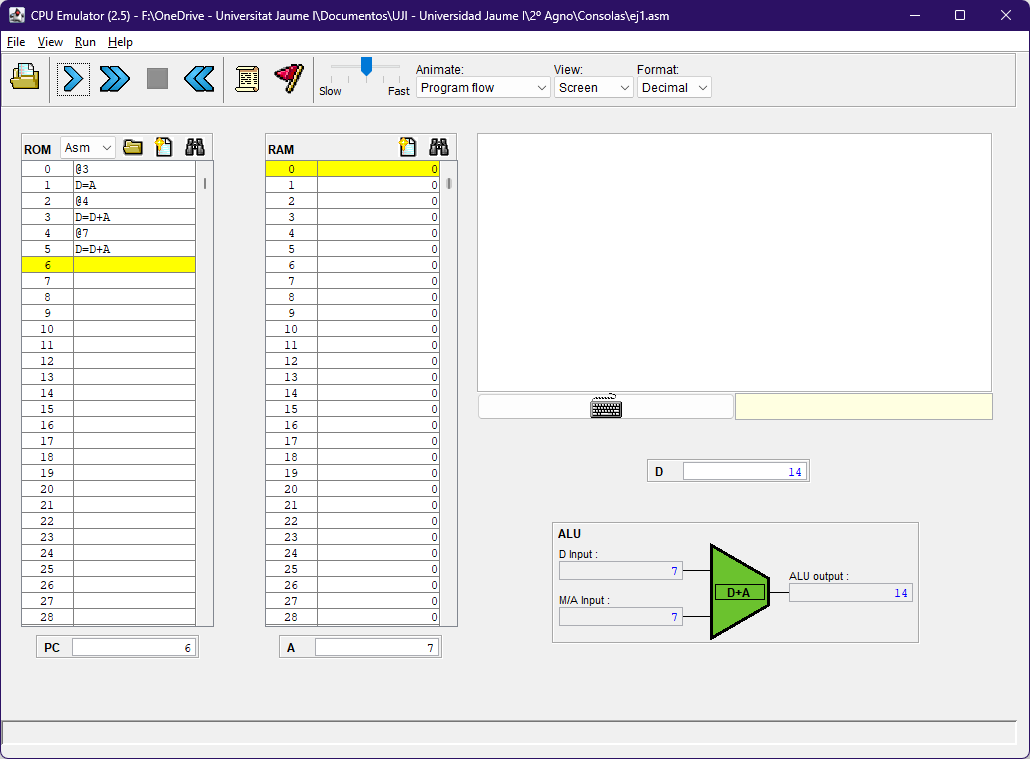
\includegraphics[width=1\linewidth]{Imagenes/ej1}
				\label{fig:ej1}
			\end{figure}

		\newpage
		\subsection{Ejercicio 2}
			\begin{lstlisting}
	// Suma de 3+4+7 en binario
	0000000000000011 // Produce en A = 3, poner el numero sin 111 al princpio, produce un numero binario
	1110110000010000 // Pone c1 y c2 activados = computar en A (0110000)... d2 activado (010), destino = D
	0000000000000100 // Guarda en A = 4
	1110000010010000 // Guarda en D (d2 activado (010)) la suma de D + A (c5 activado 000010)
	0000000000000111 // Guarda en A = 7
	1110000010010000 // Guarda en D (d2 activado (010)) la suma de D + A (c5 activado 000010)
			\end{lstlisting}

			\begin{figure}[H]
				\centering
				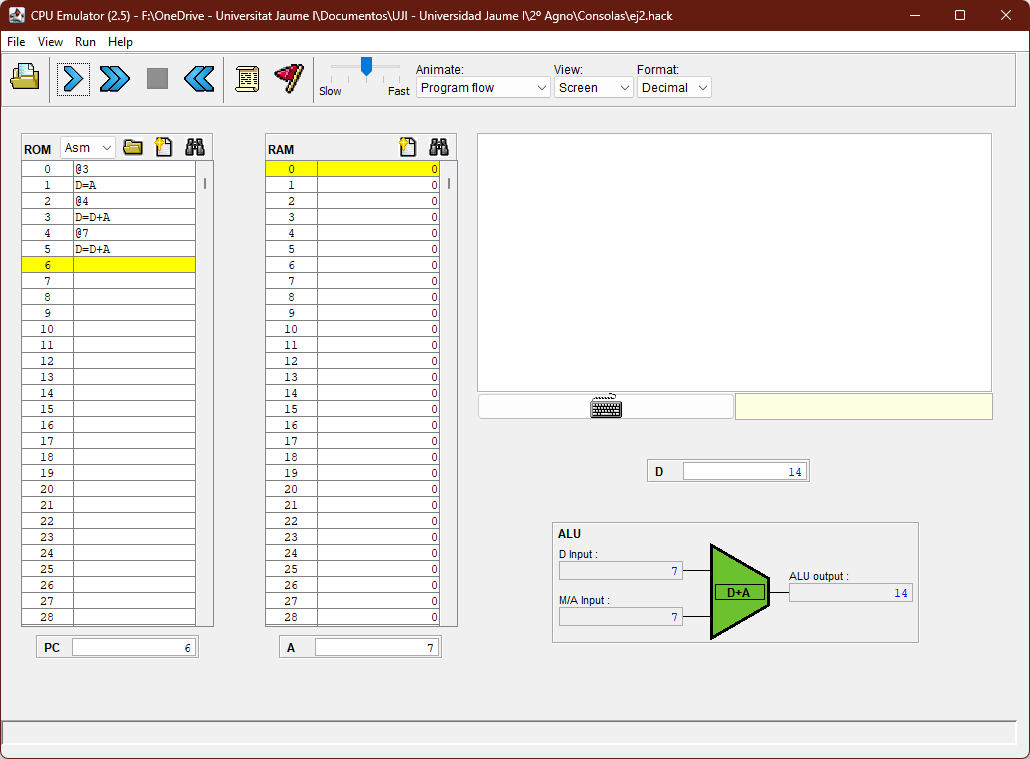
\includegraphics[width=1\linewidth]{Imagenes/ej2}
				\label{fig:ej2}
			\end{figure}
		\newpage
		\subsection{Ejercicio 3}
			\begin{figure}[H]
				\centering
				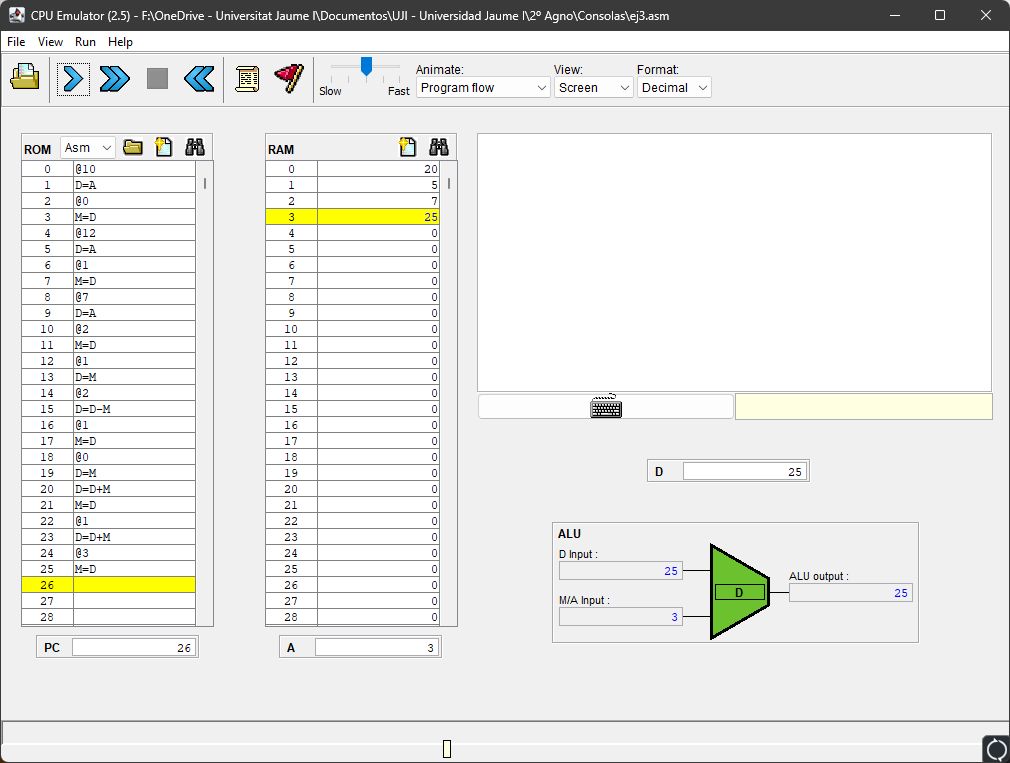
\includegraphics[width=1\linewidth]{Imagenes/ej3}
				\label{fig:ej3}
			\end{figure}

			\newpage
			\begin{lstlisting}

		// Operacion
		// x = 10 ; y = 12 ; z = 7
		// x = y - z + 2 * x

		// Ponemos cada valor en una "slot" de memoria
		@10
		D = A
		@0
		M = D
		@12
		D = A
		@1
		M = D
		@7
		D = A
		@2
		M = D

		// Se hace y - z y se pone su resultado en RAM[1]
		@1
		D = M
		@2
		D = D - M
		@1
		M = D

		// Se hace 2 * x ; se pone el resultado en RAM[0]
		@0
		D = M
		D = D + M
		M = D

		// Se calcula (y-z) * (2*x) ; usando los resultados de RAM[0] y RAM[1]
		// Se pone el resultado en RAM[3]
		@1
		D = D + M
		@3
		M = D
			\end{lstlisting}

\newpage

\printbibliography[title={Biliografía y agradecimientos}]
\end{document}